% ════════════════════════════════════════════
% 7. 数据可视化
% ════════════════════════════════════════════
\section{数据可视化}

全文图形采用同一套规范：白底、0.8 磅细边框、向内刻度，西文 Times New Roman、中文宋体，字号分 11、9.5、8.5 三档，配色只用深蓝（主）、红（对比）、绿与青（分类）、灰（不显著或参考），保证任意两图并排时不出现视觉冲突。图形类型按“要表达什么”选择：分布与分组差异用雨云图与小提琴图，关系用气泡矩阵与联合分布，模型结果用森林图与哑铃图，稳健性用横条区间图与系数矩阵，避免全文只用柱状图。

分组证据已在第 6.7 节以表\ref{tab:hetero}给出：主题 1 的付费系数为 0.571、区间位于全样本区间右侧，主题 3 为 0.018、区间覆盖零点，两组差异在数值上直接可读，无需另设图形。



图\ref{fig:overview}是全文结论的图形摘要，四个象限各给出一个核心数值：付费带来的净效应 40.1\%、视频相对图片的倍数 4.90、模型的解释力 $R^2=0.207$、共线处理前后的最大方差膨胀因子 143.0 与 3.23。四个数值分别对应第 6 章的效应测算、模型比较、方差分解与共线诊断，图形的作用是让读者在不读正文的情况下也能把握结论的量级与不确定性。

\begin{figure}[htbp]
  \centering
  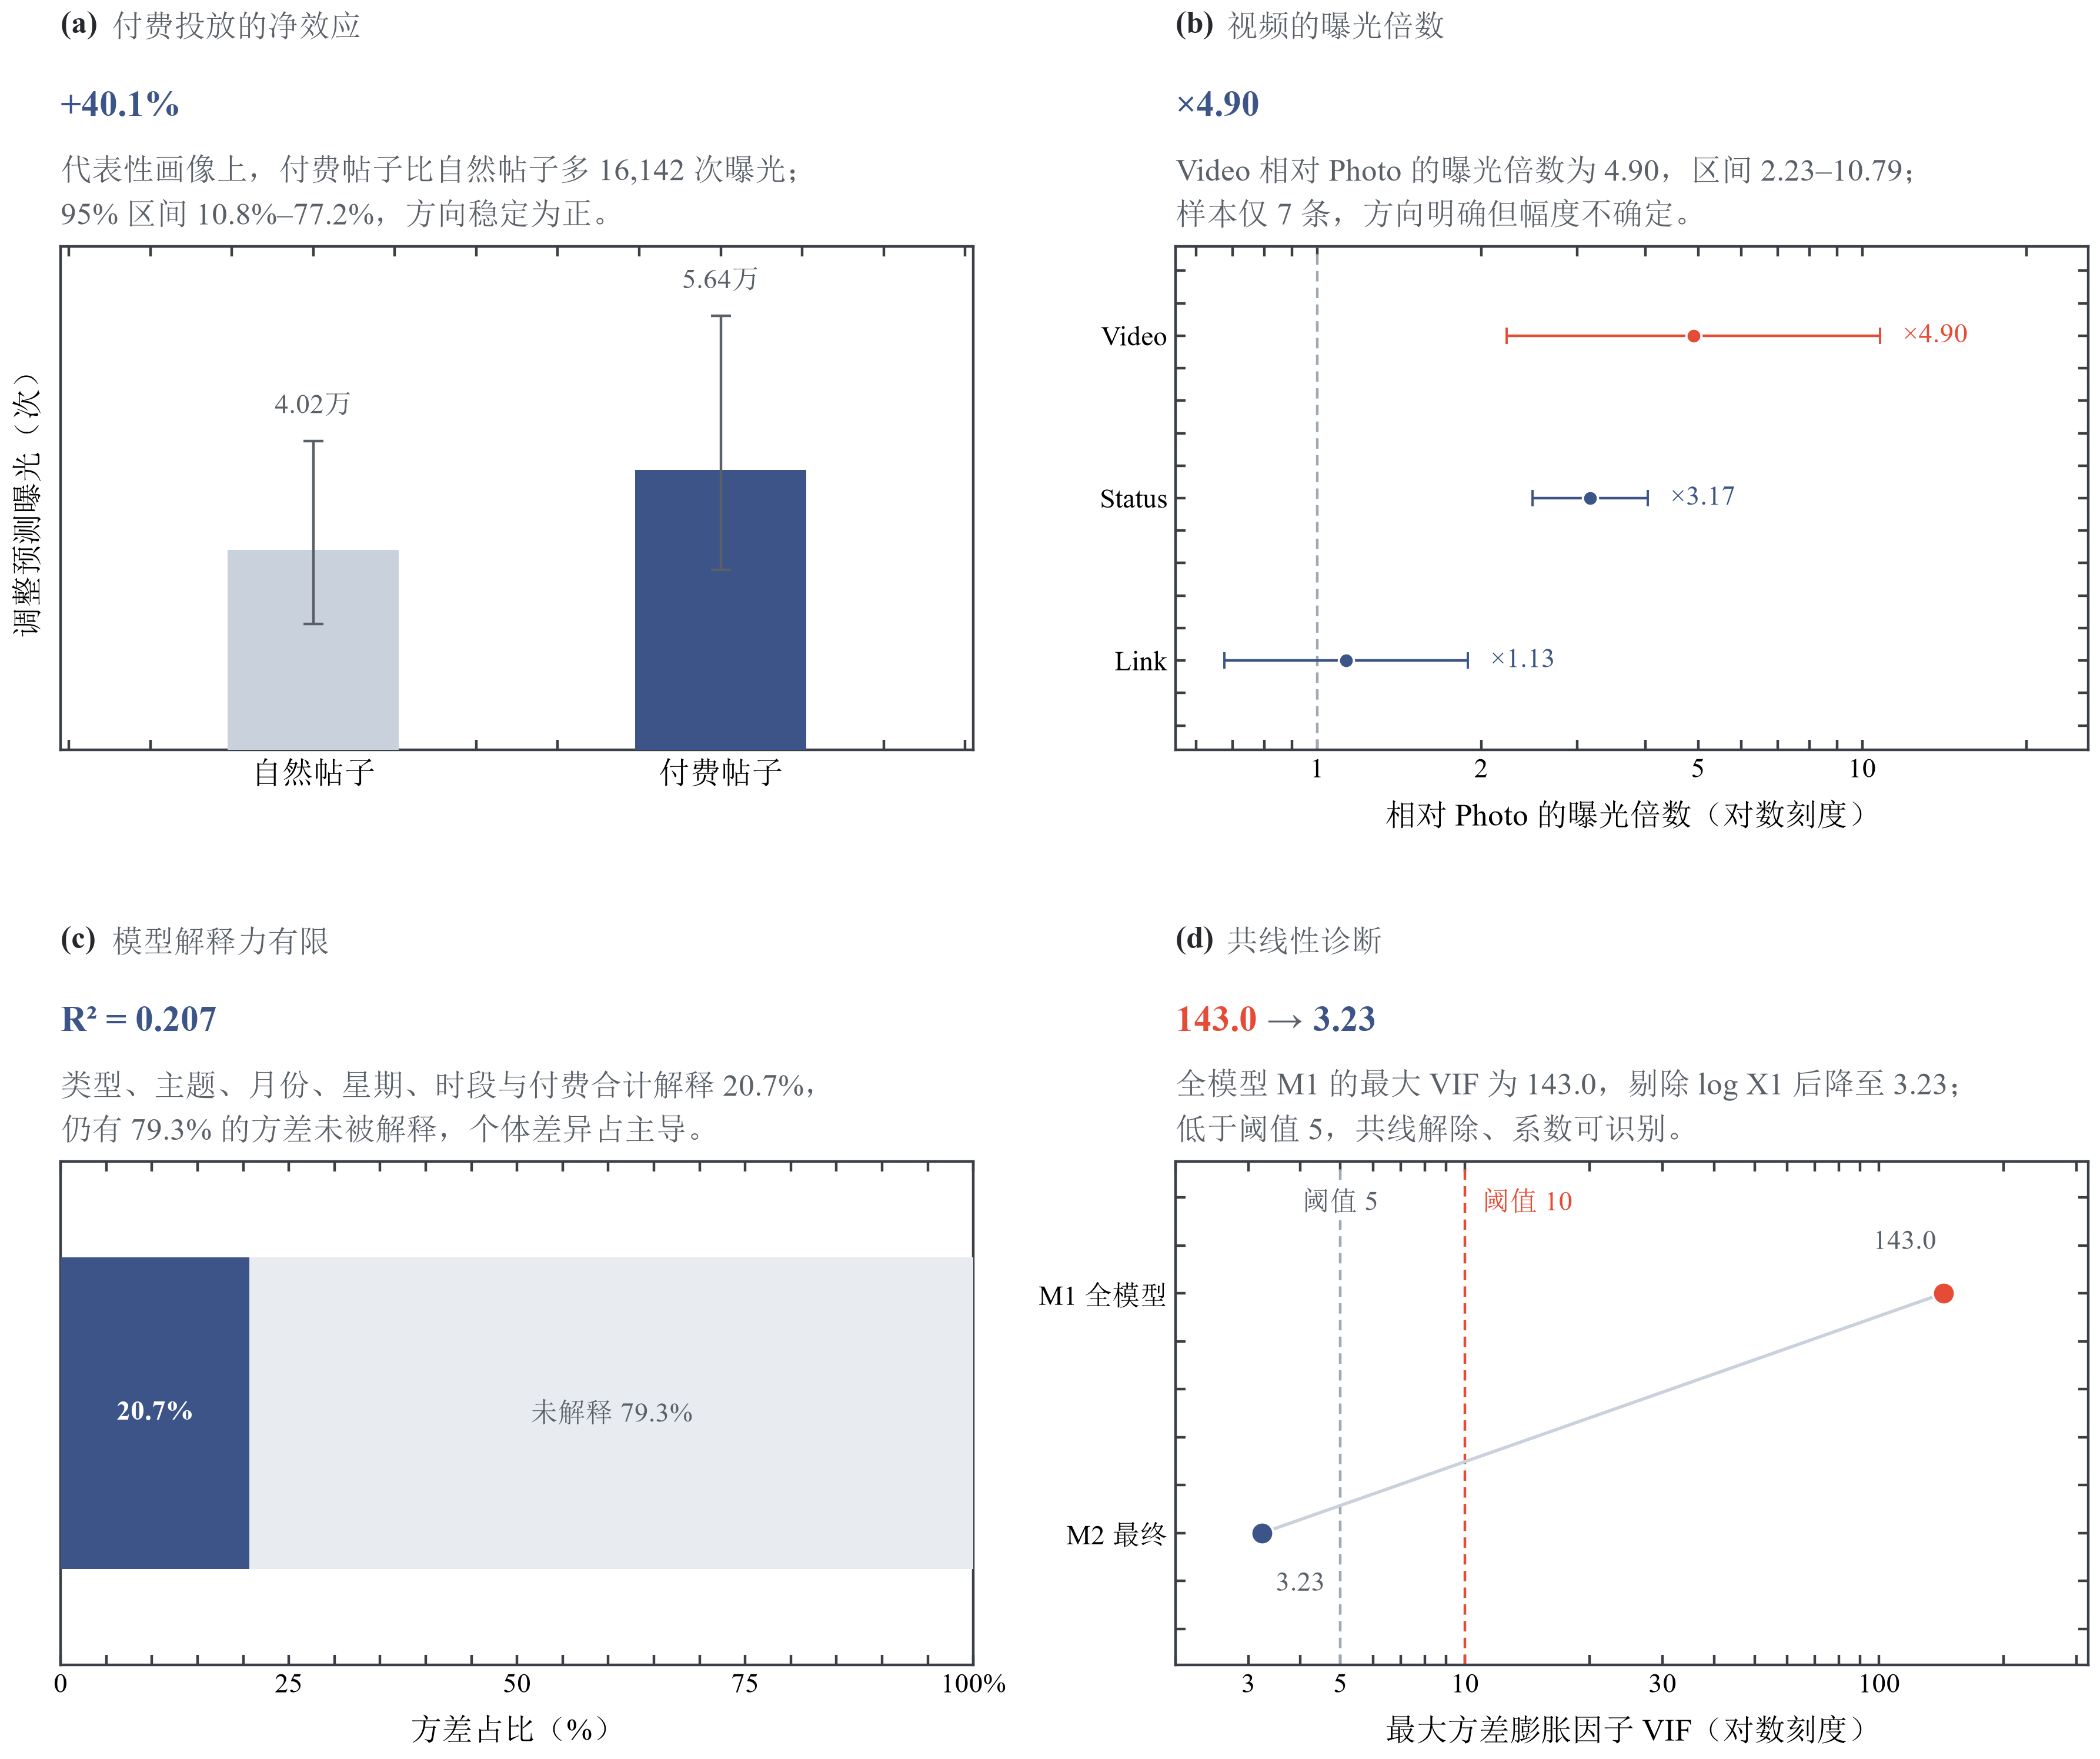
\includegraphics[width=0.70\textwidth]{../求解/临时产物/图13_核心结论总览.png}
  \caption{核心结论总览：效应、倍数、解释力与共线处理}
  \label{fig:overview}
\end{figure}
